% ---------------- RELAZIONE TIROCINIO | SMART GARDENING APP --------
\documentclass[a4paper,12pt]{report}

% ----------------------------- PREAMBLE --------------------------------------- 

\usepackage{lmodern}
\usepackage{alltt, fancyvrb, url}
\usepackage{float}
\usepackage{graphicx}
\usepackage[utf8]{inputenc}
\usepackage{hyperref}
\usepackage{amsmath,amssymb,amsthm}

\usepackage[italian]{babel}

\usepackage[italian]{cleveref}

\usepackage{comment}
\usepackage{microtype}
\usepackage{fancyhdr}

\usepackage[scaled=.92]{helvet}
\usepackage[T1]{fontenc}

\usepackage{lscape}

\usepackage{subcaption}

% hyperref settings
\hypersetup{
	colorlinks=true,
	linkcolor=black, %blue
	filecolor=magenta,      
	urlcolor=cyan,
	pdftitle={Sharelatex Example},
	bookmarks=true,
	pdfpagemode=FullScreen,
}

\usepackage{titlesec}
%\usepackage{titletoc}

\setcounter{tocdepth}{4}
\setcounter{secnumdepth}{1}

\titleformat{\section}{\normalfont\Large\bfseries\centering}{}{0pt}{} % Questo serve per togliere il numero dalla section

% ----------------------------- PREAMBLE END -----------------------------------

\makeindex

\title{\textbf{Tirocinio} \\[1.5ex] Smart Gardening App}
\author{Luca Rengo}

\begin{document}
	
\makeatletter
\begin{titlepage}
	\begin{center}
		
\includegraphics[width=0.7\linewidth]{images/logo/plant-icon.png}\\
		{\Huge  \@title }\\[3ex] 
		{\large  \@author}\\[3ex] 
		{\large Maggio | Giugno | Luglio | Agosto | Settembre}\\[3ex]
		{\large 2022}\\[3ex]
	\end{center}
\end{titlepage}
\makeatother
\thispagestyle{empty}
\newpage
	
%\maketitle

\tableofcontents

\newpage

% \input: import the commands from filename.tex to target file.

% \include: does a \clearpage and does an \input.
	
% ============================== INTRODUZIONE =========================================
	
\section{Introduzione}

\textsf{\small L'obiettivo del tirocinio era quello di sviluppare un'applicazione mobile per il monitoraggio della qualità dell'aria dell'ambiente attraverso dei sensori e la cura delle piante.}

\textsf{\small Il tirocinio si è svolto dal 23-24 maggio ai primi di ottobre 2022.}

% ============================== TECNOLOGIE ===========================================

\section{Tecnologie}

\textsf{\small Le tecnologie utilizzate sono state: \emph{Flutter}, framework per la creazione dell'app, \emph{dart}, il linguaggio del framework, \emph{TensorFlowLite} che è una libreria per il machine learning che ho usato per il riconoscimento delle piante e delle malattie di queste, \emph{Postman} che è un tool per il testing delle API che ho utilizzato per interfacciarmi con le api: \href{open.plantbook.io}{Plantbook} e \href{https://dev.netatmo.com/apidocumentation/oauth}{Netatmo API} attraverso il protocollo standard \emph{OAuth2}.} 
\textsf{\small Ho usufruito del sito \href{https://teachablemachine.withgoogle.com/}{Teachable Machine} per creare il modello tflite delle piante e quello delle loro malattie.}

% ============================== ATTIVITA' ============================================

\section{Attività}

\textsf{\small Qui, di seguito vado a presentare le varie \emph{features} e i vari \emph{screens}, sia con tema chiaro che scuro e con lingua italiana e inglese, dell'applicazione: }

\subsection{Splash Screen}

\textsf{\small Questo è lo screen di apertura dell'applicazione che dà il benvenuto all'utente.}
\textsf{\small Può essere chiaro o scuro, a seconda del tema selezionato.}

\begin{figure}[H]

\begin{subfigure}{0.3\textwidth}
	
\includegraphics[width=\textwidth]{./images/splash/splash_screen.png}
	\caption{Splash Screen}
	\label{fig:splash_screen}
\end{subfigure}
\hfill
\begin{subfigure}{0.3\textwidth}
	
\includegraphics[width=\textwidth]{./images/splash/splash_screen_dark.png}
	\caption{Splash Screen Dark}
	\label{fig:splash_screen_dark}
\end{subfigure}

\end{figure}

\subsection{OnBoarding}

\textsf{\small Dopo lo Splash Screen, c'è una piccola introduzione alle funzionalità dell'app.}
\textsf{\small Queste schermate verranno mostrate la prima volta e poi verranno disabilitate, a meno che l'utente modifichi l'impostazione nel \emph{Settings Screen}.}

\begin{figure}[H]
	
\begin{subfigure}{0.3\textwidth} %TODO: volendo metterli tutti a 0.2, oppure no, va bene anche così
	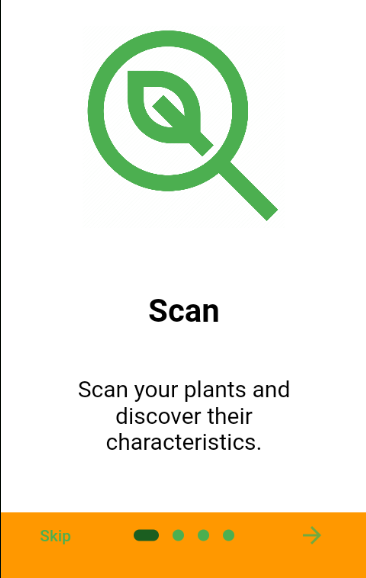
\includegraphics[width=\textwidth]{./images/onboarding/onboarding_screen0.png}
	\caption{OnBoarding Screen Pagina 1}
	\label{fig:onboarding}
\end{subfigure}
\hfill
\begin{subfigure}{0.3\textwidth}
	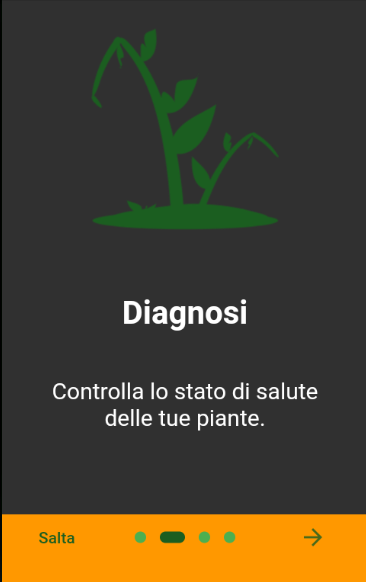
\includegraphics[width=\textwidth]{./images/onboarding/onboarding_screen1_dark.png}
	\caption{OnBoarding Screen Pagina 2}
	\label{fig:onboarding1}
\end{subfigure}
\hfill
\begin{subfigure}{0.3\textwidth}
	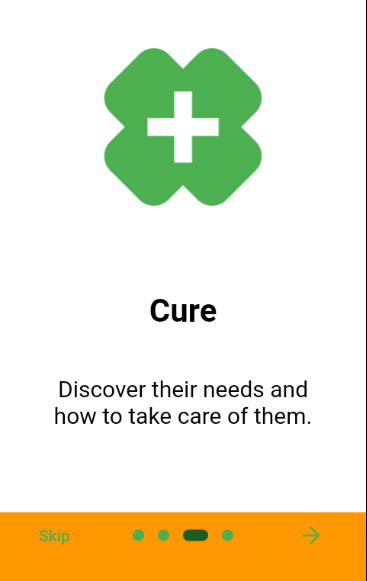
\includegraphics[width=\textwidth]{./images/onboarding/onboarding_screen2.png}
	\caption{OnBoarding Screen Pagina 3}
	\label{fig:onboarding2}
\end{subfigure}
\hfill
\begin{subfigure}{0.3\textwidth}
	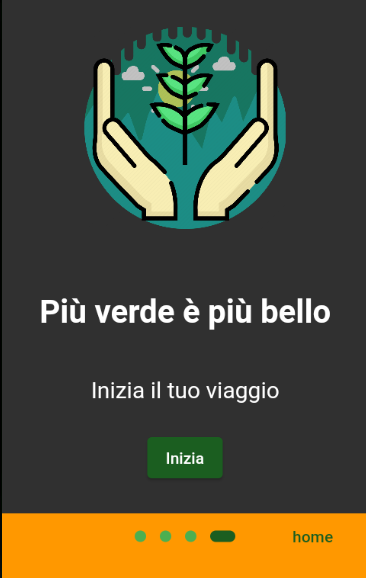
\includegraphics[width=\textwidth]{./images/onboarding/onboarding_screen3_dark.png}
	\caption{OnBoarding Screen Pagina 4}
	\label{fig:onboarding3}
\end{subfigure}
\end{figure}

\subsection{Homepage}

\textsf{\small La Homepage è la pagina principale dell'applicazione, da questa è possibile raggiungere tutte le altre pagine.}
\textsf{\small In basso è presente una \emph{BottomNavigationBar} che consente un rapido spostamento tra le pagine.}
\textsf{\small In alto a sinistra, cliccando sull'icona menù si potrà accedere al \emph{NavigationDrawer}.}
\textsf{\small In alto a destra, con l'icona della camera, si accede alla schermata della scansione delle piante, mentre con l'icona della bandierina sarà possibile modificare la lingua dell'intera app in tempo reale, senza doverla riavviare.}
\textsf{\small E infine, i pulsanti al centro dello schermo mostrano le varie attività.}

\begin{figure}[ht] 
	\centering
	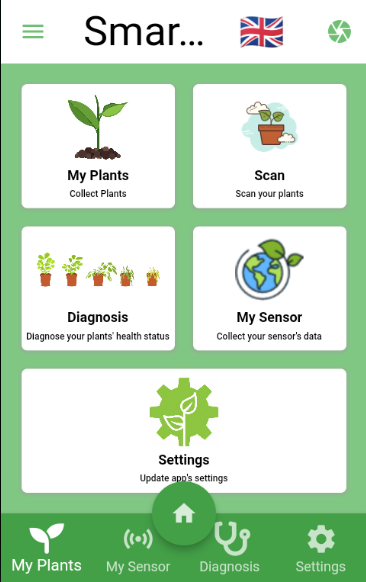
\includegraphics[width=.5\textwidth, height=.5\textheight, keepaspectratio]{./images/home/home_screen.png}
	\caption{Homepage}
	\label{fig:homepage}
\end{figure}

\subsection{Navigation Drawer}

%\label{navigation_drawer}

\textsf{\small Questo è un pannello menù che permette di visitare tutte le pagine dell'app, anche quelle non presenti nella \emph{HomePage} e nella \emph{BottomNavigationBar}.}

\begin{figure}[H]
	
	\begin{subfigure}{0.3\textwidth}
		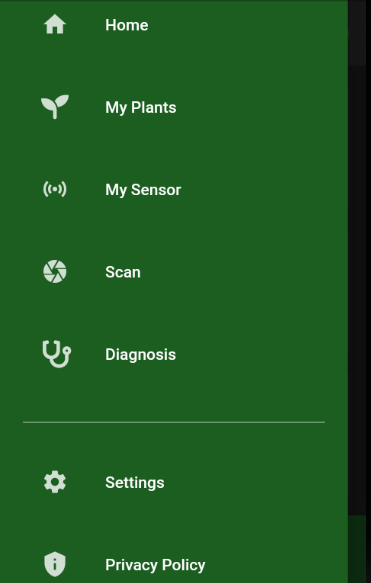
\includegraphics[width=\textwidth]{./images/navigation_drawer/navigation_drawer.png}
		\caption{Navigation Drawer}
		\label{fig:navigation_drawer}
	\end{subfigure}
	\hfill
	\begin{subfigure}{0.3\textwidth}
		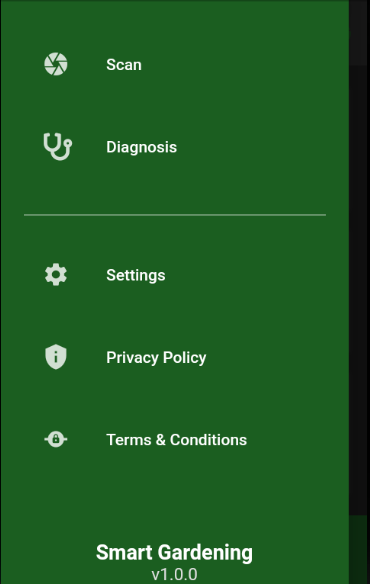
\includegraphics[width=\textwidth]{./images/navigation_drawer/navigation_drawer2.png}
		\caption{Navigation Drawer}
		\label{fig:navigation_drawer2}
	\end{subfigure}
\end{figure}

\subsection{Scan Screen \& Scan Result Screen}

%\textsf{\small Si accede a questa pagina attraverso l'icona della camera in alto a destra nella \emph{Homepage}.}
\textsf{\small In questa schermata è possibile premere due pulsanti: uno per caricare un'immagine dalla galleria e l'altro per caricarla dalla fotocamera scattando una foto.}
\textsf{\small Una volta scelta l'immagine questa andrà eseguita sul modello di piante tflite che riconoscerà di quale pianta si tratta.}
\textsf{\small Nel modello sono presenti 58 piante da giardino comuni.}
\textsf{\small Se la pianta non è presente, verrà mostrato, sullo schermo, un errore.}

\begin{figure}[ht] 
	\centering
	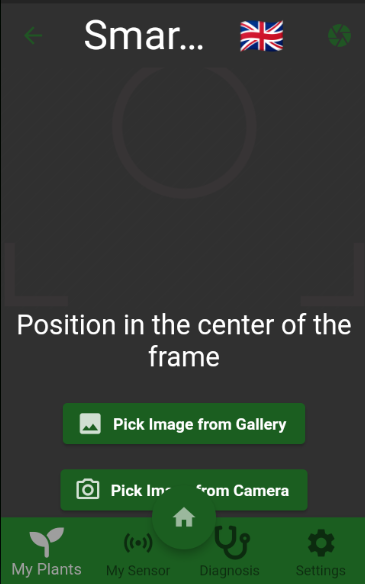
\includegraphics[width=.3\textwidth, height=.3\textheight, keepaspectratio]{./images/scan/scan_screen.png}
	\caption{Scan Screen}
	\label{fig:scan}
\end{figure}

\textsf{\small Ricavata la pianta, questa verrà passata alla schermata di risultato che ne mostrerà le caratteristiche e l'immagine caricata dall'utente.}
\textsf{\small Se l'utente preme il pulsante con l'icona '+', allora questa pianta appena scannerizzata verrebbe aggiunta al database delle piante e l'utente potrebbe visionarla quando vuole nella schermata \emph{MyPlants} (Le mie piante).}
\textsf{\small Se l'operazione è andata a buon fine, allora un messaggio in verde verrà mostrato sullo schermo per informare l'utente che l'operazione è stata eseguita con successo, altrimenti un messaggio in rosso.}

\begin{figure}[H]
	
	\begin{subfigure}{0.3\textwidth}
		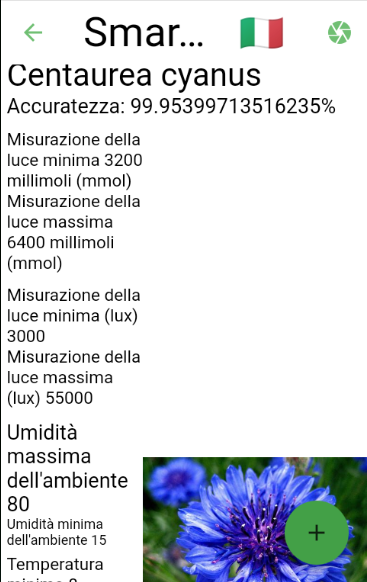
\includegraphics[width=\textwidth]{./images/scan_result/scan_result_screen.png}
		\caption{Scan Result Screen}
		\label{fig:scan_result}
	\end{subfigure}
	\hfill
	\begin{subfigure}{0.3\textwidth}
		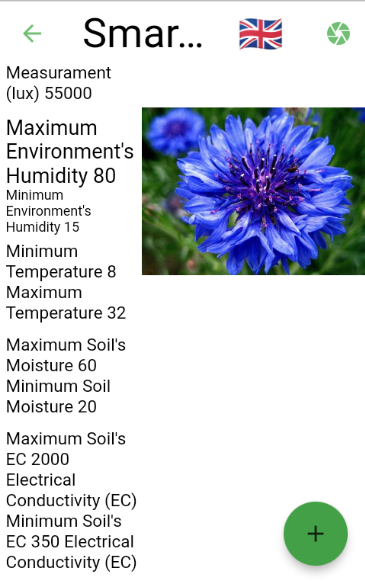
\includegraphics[width=\textwidth]{./images/scan_result/scan_result_screen2.png}
		\caption{Scan Result Screen 2}
		\label{fig:scan_result2}
	\end{subfigure}
	\hfill
	\begin{subfigure}{0.3\textwidth}
		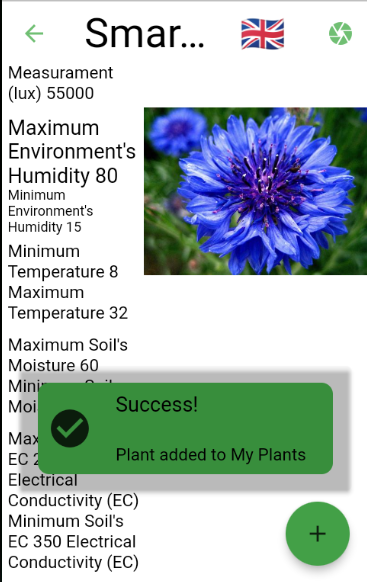
\includegraphics[width=\textwidth]{./images/scan_result/scan_result_screen3.png}
		\caption{Scan Result Screen 3}
		\label{fig:scan_result3}
	\end{subfigure}
\end{figure}

\subsection{My Plants \& My Plants Details Screens}

\textsf{\small Questa schermata mostra tutte le piante salvate nel database dall'utente dopo averle scannerizzate.}
\textsf{\small L'utente può cliccare su queste per vederne i dettagli oppure cliccare sull'icona del 'cestino' per eliminarle dal database e dalla schermata.}
\textsf{\small Se l'operazione è stata eseguita con successo un messaggio in verde di successo verrà mostrato.}
\textsf{\small Come tutte le schermate è possibile cambiare lingua del testo in tempo reale.}

\begin{figure}[H]	
	\begin{subfigure}{0.3\textwidth}
		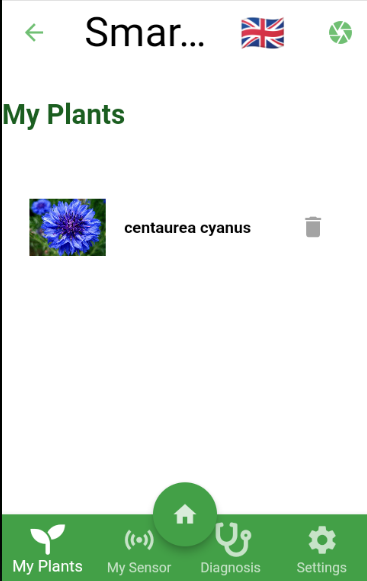
\includegraphics[width=\textwidth]{./images/my_plants/my_plants_screen2.png}
		\caption{My Plants Screen 0}
		\label{fig:my_plants}
	\end{subfigure}
	\hfill
	\begin{subfigure}{0.3\textwidth}
		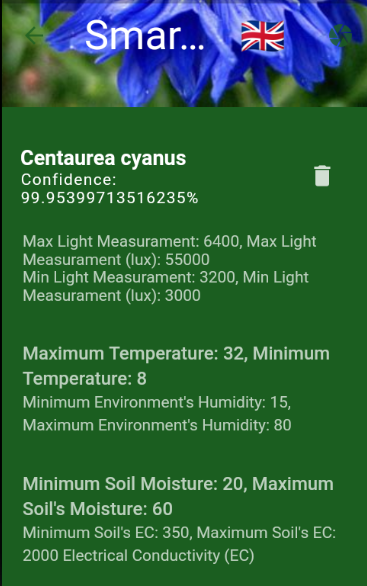
\includegraphics[width=\textwidth]{./images/my_plants/my_plants_details_screen.png}
		\caption{My Plants Details Screen 1}
		\label{fig:my_plants1}
	\end{subfigure}
	\hfill
	\begin{subfigure}{0.3\textwidth}
		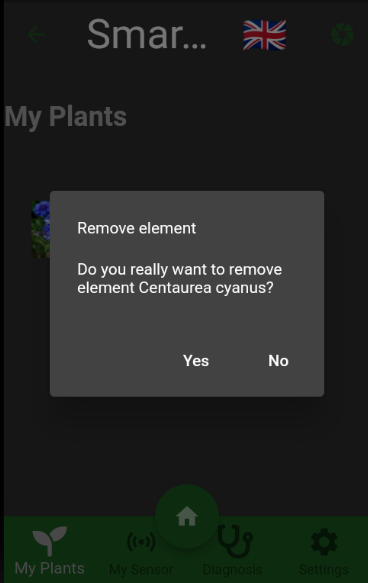
\includegraphics[width=\textwidth]{./images/my_plants/my_plants_screen3_remove.png}
		\caption{My Plants Screen Remove}
		\label{fig:my_plants_remove}
	\end{subfigure}
	\hfill
	\begin{subfigure}{0.3\textwidth}
		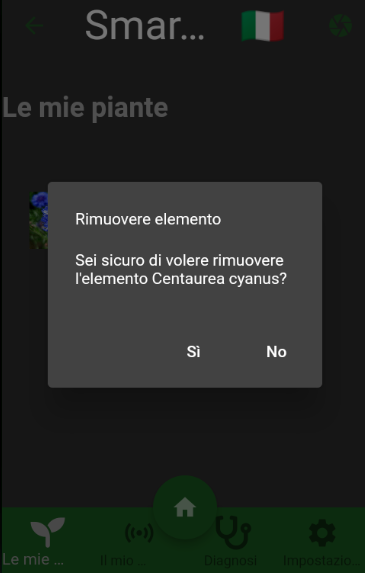
\includegraphics[width=\textwidth]{./images/my_plants/my_plants_screen3_remove2.png}
		\caption{My Plants Screen Remove 2}
		\label{fig:my_plants_remove2}
	\end{subfigure}
	\hfill
	\begin{subfigure}{0.3\textwidth}
		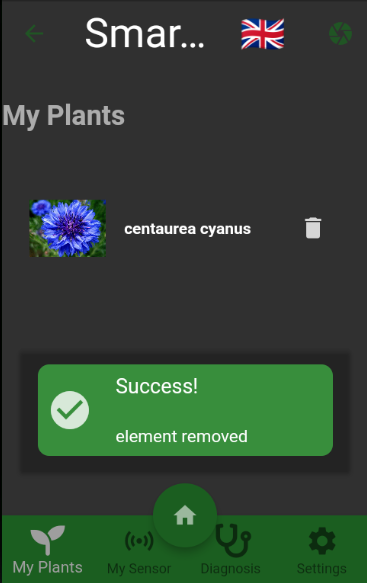
\includegraphics[width=\textwidth]{./images/my_plants/my_plants_screen3_remove3.png}
		\caption{My Plants Screen Remove 3}
		\label{fig:my_plants_remove3}
	\end{subfigure}
	\hfill
	\begin{subfigure}{0.3\textwidth}
		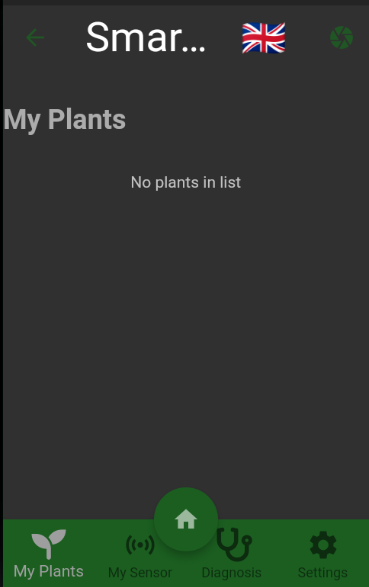
\includegraphics[width=\textwidth]{./images/my_plants/my_plants_screen.png}
		\caption{My Plants Screen List Empty}
		\label{fig:my_plants_list_empty}
	\end{subfigure}
\end{figure}

\subsection{Diagnosis Screen}

\textsf{\small In questo screen, come nello screen dello \emph{Scan}, possiamo caricare una foto, nelle stesse identiche procedure di prima e queste verranno eseguite sul modello che ne ricaverà la malattia della pianta, se ne ha, altrimenti indicherà che è sana.}
\textsf{\small Il modello delle malattie presenta 60 malattie diverse delle piante.}

\begin{figure}[ht] 
	\centering
	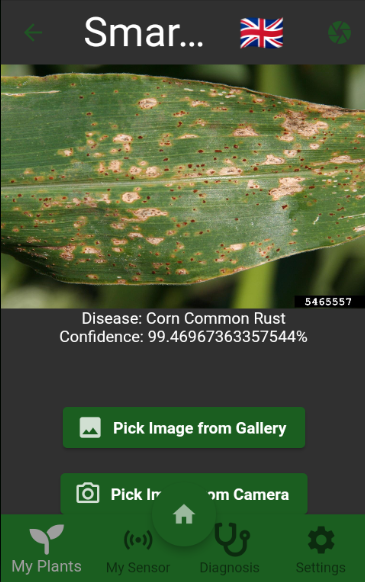
\includegraphics[width=.3\textwidth, height=.3\textheight, keepaspectratio]{./images/diagnosis/diagnosis_screen.png}
	\caption{Diagnosis Screen}
	\label{fig:diagnosis}
\end{figure}

\subsection{My Sensor Screen}

\textsf{\small In questa schermata, dopo aver inserito un \emph{device\_id} che è il mac address del sensore Netatmo, verranno mostrati i dati di questo.}
\textsf{\small Se ne si inserisce uno errato o se si cerca di ottenere i dati senza aver inserito nulla nel campo di testo, allora verrà mostrato un errore.}
\textsf{\small Se il \emph{device\_id} è corretto e si riescono a recuperare i dati dall'API, allora un messaggio di successo verrà mostrato.}

\begin{figure}[H]	
	\begin{subfigure}{0.3\textwidth}
		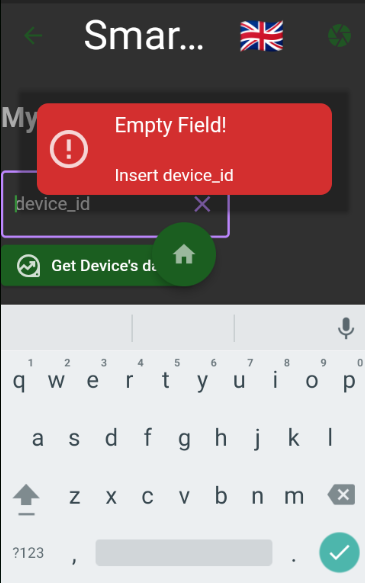
\includegraphics[width=\textwidth]{./images/my_sensor/my_sensor_screen.png}
		\caption{My Sensor Screen}
		\label{fig:my_sensor}
	\end{subfigure}
	\hfill
	\begin{subfigure}{0.3\textwidth}
		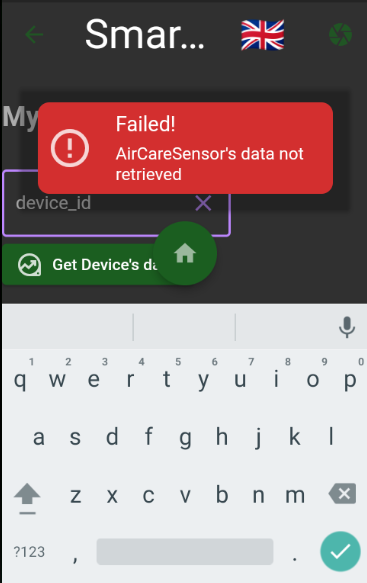
\includegraphics[width=\textwidth]{./images/my_sensor/my_sensor_screen2.png}
		\caption{My Sensor Screen 2}
		\label{fig:my_sensor2}
	\end{subfigure}
	\begin{comment}
	\hfill
	\begin{subfigure}{0.3\textwidth}
		\includegraphics[width=\textwidth]{./images/my_sensor/my_sensor_screen3.png}
		\caption{My Sensor Screen 3}
		\label{fig:my_sensor3}
	\end{subfigure}
	\end{comment}
	\hfill
	\begin{subfigure}{0.3\textwidth}
		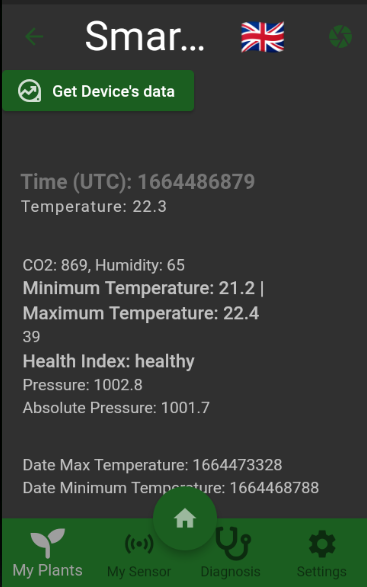
\includegraphics[width=\textwidth]{./images/my_sensor/my_sensor_screen5.png}
		\caption{My Sensor Screen 3} %4
		\label{fig:my_sensor4}
	\end{subfigure}
\end{figure}

\subsection{Settings Screen}

\textsf{\small Nel settings screen è possibile modificare: lingua, tema, visibilità delle pagine di benvenuto.}
\textsf{\small Se l'utente le modifica, queste verranno cambiate, ma verranno salvate solamente se l'utente avrà cliccato sul pulsante 'SALVA'.}
\textsf{\small Se è la prima volta che l'utente apre l'applicazione, il tema e la lingua verranno settati in base a quelli del suo dispositivo, se possibile.}
\textsf{\small Se l'utente ha salvato delle impostazioni, la volta dopo che apre l'applicazione queste verranno caricate dalle preferenze dell'utente e non dalle impostazioni del suo sistema.}
\textsf{\small Se l'utente clicca il pulsante 'RESET', allora le impostazioni di default verranno salvate nelle sue preferenze, ovvero, lingua: inglese, tema: chiaro, pagine di benvenuto: on.}

\begin{figure}[H]	
	\begin{subfigure}{0.3\textwidth}
		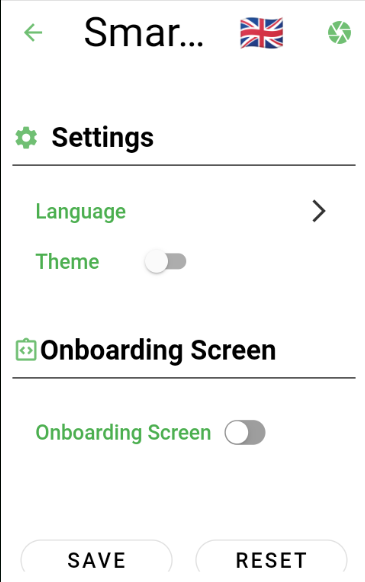
\includegraphics[width=\textwidth]{./images/settings/settings_screen.png}
		\caption{Settings Screen}
		\label{fig:settings}
	\end{subfigure}
	\hfill
	\begin{subfigure}{0.3\textwidth}
		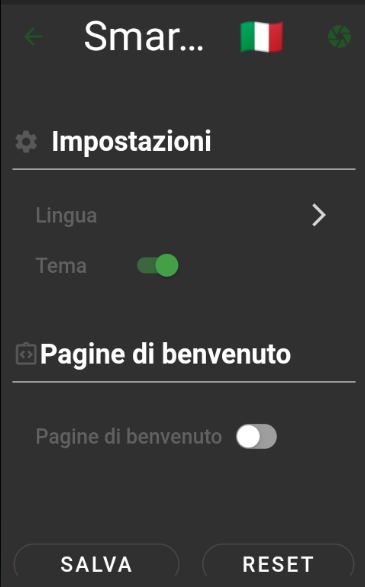
\includegraphics[width=\textwidth]{./images/settings/settings_screen2.png}
		\caption{Settings Screen 2}
		\label{fig:settings2}
	\end{subfigure}
		\hfill
		\begin{subfigure}{0.3\textwidth}
			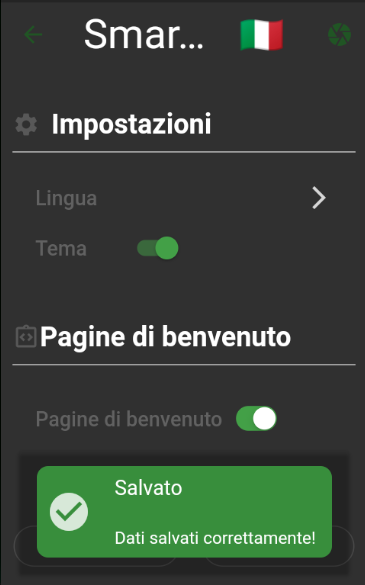
\includegraphics[width=\textwidth]{./images/settings/settings_screen_saved.png}
			\caption{Settings Screen Saved}
			\label{fig:settings_saved}
		\end{subfigure}
	\hfill
	\begin{subfigure}{0.3\textwidth}
		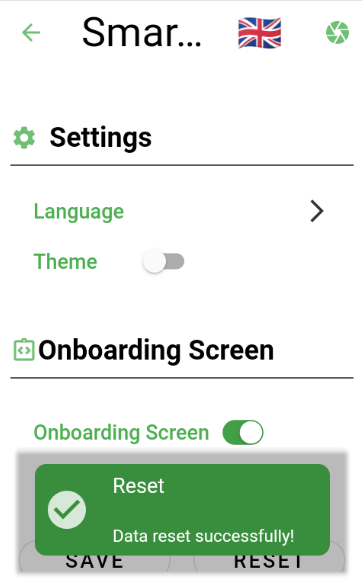
\includegraphics[width=\textwidth]{./images/settings/settings_screen_reset.png}
		\caption{Settings Screen Reset} %4
		\label{fig:settings_reset}
	\end{subfigure}
\end{figure}

\textsf{\small Per entrambe queste operazioni verrà mostrato un messaggio di successo, se saranno andate a buon fine.}

\subsection{Privacy Policy and Terms \& Conditions Screens}

\textsf{\small Infine, le ultime due pagine, accessibili solamente attraverso il \emph{Navigation Drawer}, sono l'Informativa sulla Privacy e Termini \& Condizioni.}

\begin{figure}[H]	
	\begin{subfigure}{0.3\textwidth}
		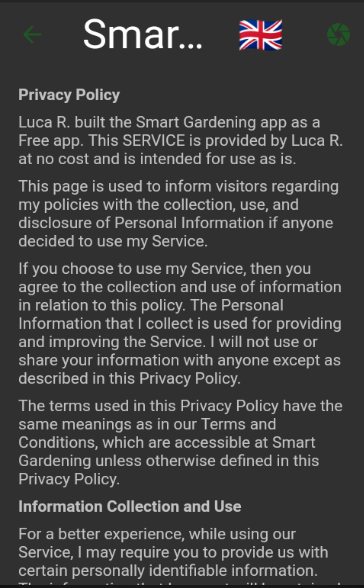
\includegraphics[width=\textwidth]{./images/privacy_policy/privacy_policy_screen.png}
		\caption{Privacy Policy}
		\label{fig:privacy_policy}
	\end{subfigure}
	\hfill
	\begin{subfigure}{0.3\textwidth}
		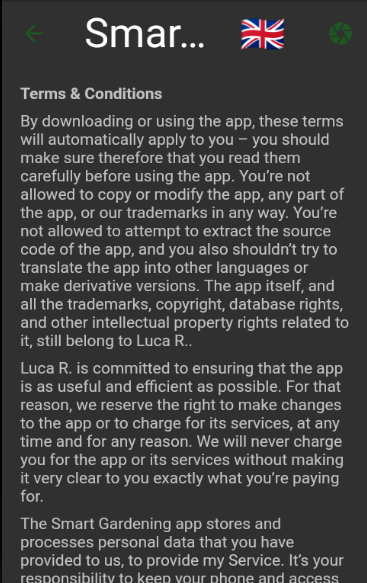
\includegraphics[width=\textwidth]{./images/terms_and_conditions/terms_and_conditions_screen.png}
		\caption{Terms \& Conditions}
		\label{fig:terms_and_conditions}
	\end{subfigure}
\end{figure}
	
% ============================== GUIDA UTENTE =========================================
	
\newpage

\section{Guida utente}

\textsf{\small Qui, di seguito verranno indicate le procedure e le istruzioni da eseguire per poter avviare correttamente l'applicazione: }

\begin{itemize}
	\item \textsf{\small Installare l'apk sul proprio dispositivo Android.}
	\item \textsf{\small Oppure installare .ipa sul proprio dispositivo iOS.}
\end{itemize}

\textsf{\small Se si vuole modificare il codice, invece, occorrerà:}

\begin{itemize}
	\item \textsf{\small Flutter 2.10.5}
	\item \textsf{\small Nel file \emph{plant\_api.dart} nella directory \emph{/lib/api/plant\_api/} per potersi collegare con l'API OpenPlantBook, occorrerà aggiungere: }
	\begin{itemize}
		\item \textsf{\small clientId}
		\item \textsf{\small clientSecret}
	\end{itemize}
	\item \textsf{\small Nel file \emph{sensor\_api.dart} che si trova in \emph{/lib/api/sensor\_api/} sarà necessario, per potersi interfacciare con l'API di Netatmo, inserire: }
	\begin{itemize}
		\item \textsf{\small clientId}
		\item \textsf{\small clientSecret}
		\item \textsf{\small email}
		\item \textsf{\small password}
	\end{itemize}
\end{itemize}

% ============================== CONCLUSIONI ==========================================

\section{Conclusioni}

\textsf{\small Questa esperienza mi è stata molto utile per migliorare la mia capacità di creare applicazioni mobile e per capire meglio l'importanza che ricoprono e svolgono le piante nel nostro ambiente.}\break

\textsf{\small Luca Rengo}

\end{document}

% ====================================================================================


